\chapter{XML in Atom}

\begin{wrapfigure}{l}{0.5\textwidth}
	\vspace{-10pt}
	\begin{center}
		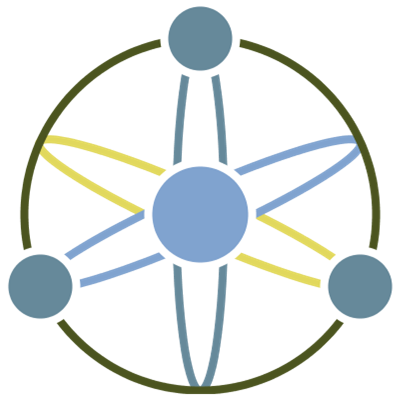
\includegraphics[scale=0.2]{atom-logo.png}
	\end{center}
	\vspace{-10pt}
	\caption{Atom logo.}
	\label{fig:atom_logo}
	\vspace{-10pt}
\end{wrapfigure}

Atom is a web syndication framework and consists of a pair of standards:

\begin{enumerate}
\item Atom Syndication Format - \href{https://tools.ietf.org/html/rfc4287}{RFC 4287}
\item Atom Publishing Protocol - \href{https://tools.ietf.org/html/rfc5023}{RFC 5023}
\end{enumerate}

An Atom feed can consist: plain text, escaped HTML, XHTML, XML, Base64-encoded binary, and references to external content as: documents, video, audio, streams etc.

Unfortunately the official website of the project no longer exists, figure \ref{fig:atom_logo} shows the original Atom project's logo.

\section{Atom Syndication Format}
"Atom is an XML-based document format" (\href{https://tools.ietf.org/html/rfc4287}{RFC 4287, page 3}). The RFC describes how a well-formed Atom document should be formatted.

\section{Atom Publishing Protocol}
This is also known as the "Atom API" and the aim of this project is to improve on and replace the existing XML-RPC-based publishing protocols \cite{xml_com}.

The Atom Publishing Protocol is based on HTTP transfer of Atom-formatted representations, formatted with the Atom Syndication Format \cite{ietf_rfc5023}.

\section{Atom vs. RSS}
Although both the Atom and the RSS standard facilitate the same (a news feed), there are some key differences as shown in table \ref{tab:atomvsrss} below.

\begin{table}[h]
	\begin{tabular}{|l|l|}
	\hline
	Atom & RSS \\ \hline
	Indication of content type & No indication of content type \\
	RFC3339 timestamps & RFC822 timestamps \\
	Supports language ids per readable item & Supports language identifier per article \\
	Reusable elements out of context & Non-reusable elements out of context \\
	\hline
	\end{tabular}
	\caption{Atom vs. RSS}
	\label{tab:atomvsrss}
\end{table}

\section{Atom Document Example}
Atom feeds contain one or more entry sections below the main meta-data section.

\begin{lstlisting}[style=xml, frame=single, caption={feed.xml}]
<?xml version="1.0" encoding="utf-8"?>
<feed xmlns="http://www.w3.org/2005/Atom">

   <title>Example Feed</title>
   <link href="http://example.org/"/>
   <updated>2003-12-13T18:30:02Z</updated>
   <author>
     <name>John Doe</name>
   </author>
   <id>urn:uuid:60a76c80-d399-11d9-b93C-0003939e0af6</id>

   <entry>
     <title>Atom-Powered Robots Run Amok</title>
     <link href="http://example.org/2003/12/13/atom03"/>
     <id>urn:uuid:1225c695-cfb8-4ebb-aaaa-80da344efa6a</id>
     <updated>2003-12-13T18:30:02Z</updated>
     <summary>Some text.</summary>
   </entry>

</feed>
\end{lstlisting}

\subsection{Required feed elements}
The following tags are mandatory when creating an Atom message:
\begin{itemize}
  \item \textbf{id} - Unique and permanent URI identifying the feed
  \item \textbf{title} - Title for the feed
  \item \textbf{updated} - Last time feed was modified
  \item \textbf{author} - At least one, can be more
  \item \textbf{link} - Link to related Web page
\end{itemize}

Optional elements and can be looked found \href{http://www.atomenabled.org/developers/syndication/#optionalEntryElements}{here}. These optionals include details such as initial publication dates and copyright information.

%\end{document}
